\label{chapter:refactoring}
\chapter{Improving Software Metrics and Refactoring}
In Chapter \ref{chapter:problem-description}, the huge accumulated amount of technical debt in the system has been highlighted. A new robust and future-proof architecture has been proposed in Section \ref{chapter:architecture}. In this Chapter, the most important activities during the span of this thesis work will be presented. This includes a developer-friendly REST API and, a modern, simplistic and user-friendly grahical user interface and major important modifications to the available testing framework.

\section{General Overview and Statistics}
According to GitHub, 155 Pull Requests have been accepted, which account for a total of 401 commits. In total, 27.659 lines have been added and 12.581 lines have been removed. 765 files have been modified. These statistics excludes the removal of \emph{wxPython} GUI code which account for 12.429 deletions.

\section{Improving tests and testability}
The most fundamental way to verify the correctness of software detect issues as soon as possible in the development cycles, is by having an exhaustive test suite. As described in Chapter \ref{chapter:problem-description}, the current test suite is plagued with unstable and non-functional tests. This section will discuss the performed work to strengthen and stabilize the test suite.

\subsection{Improving Code Coverage}
Code coverage is defined as the percentage of source code that is covered by at least one test in the test suite. Our continuous integration environment offers tools to track the code coverage over time. After each automated test suite execution a comprehensive report with detailed information about the code coverage is generated. The reported metrics by this report is not very accurate since some third-party libraries are included, such as the VLC bindings and \emph{pymdht}, our used implementation to fetch peers from the Distributed Hash Table (DHT). Also, the code coverage of Dispersy is included in these reports while Dispersy is considered as a separate engineering project.\\\\
Improving the code coverage has been done by writing small unit tests where we are using mocked objects to have better control over the system we are testing. Using mocking in Tribler is a necessary since some components have many other dependencies that are hard to keep under control without using custom, controlled objects. Libtorrent is a good example of this. During this thesis, many unit tests have been written as can be seen in Figure x where the number of unit tests over time is presented. Writing tests makes a developer more aware of the written code and can be a good way to get familiar with an unknown system. Due to this, various bugs have been solved during the process of writing additional tests.

\begin{figure}[h!]
	\centering
	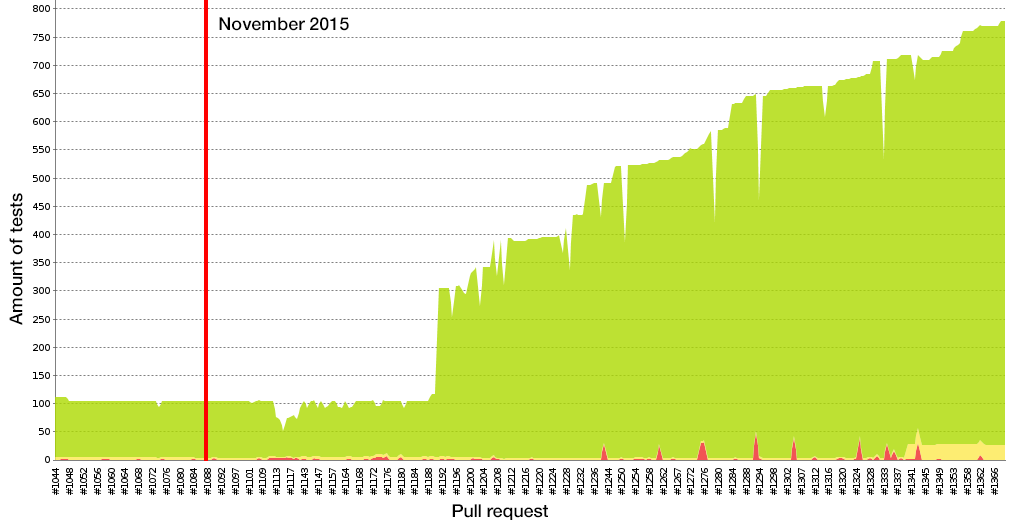
\includegraphics[width=0.8\columnwidth]{images/improving_qa/test_trend}
	\caption{The number of tests over time.}
	\label{fig:importgraph-qt-gui}
\end{figure}

In Chapter \ref{chapter:problem-description}, Figure \ref{fig:tests-ratio-tribler} we presented the ratio between the number of code lines in the tests package and the amount of other code lines over time. Together with the code coverage, this number can be a useful metric to developers. While one might argue that having a high code coverage in conjunction with a low TLC/PLC ratio is a desired result, it indicates that the tests are not granular enough and are actually doing many different things. A low code coverage with a high TLC/PLC ratio indicates that there are some flaws in the tests, possibly that they are testing the wrong components of the system. When starting the thesis, Tribler has a low code coverage together with a low TLC/PLC ratio\todo{beter uitleggen}.\\\\
After writing additional unit tests, removal of the old user interface and addition of the new one, the new ratio is \emph{0.16} which means that there is roughly one line of test code for six lines of other source code in Tribler. Defining a good TLC/PLC ratio is dependent on the used programming language, development methodology and application structure. Discussion on the wiki of Ward Cunningham\cite{c2tlcratio} proposes an optional ratio of 1:1, however, several other ratios have been proposed on the same page such as 2:1 and 5:1. Overall, the trend seems to be that the amount of test line code is higher than the lines of production code. An important question is whether this proposed ratio also holds for Tribler. Tribler differs from a commercial software engineering project in the sense that it is used for scientific research. When performing research, it is easy to ignore testing and focus on the results that are gathered by the system. The difficulty here is that Tribler is distributed and used by over a million of users, requiring at least some form of quality assurance. We think a better optional TLC/PLC ratio for the Tribler project might be 1:2.\\\\
To make sure that the responsibility of code coverage is not neglected in future work on Tribler, an addition check for each pull request has been added that verifies that the code contributed in the respective pull request is covered by tests. While not created by the author of this thesis, this check is an effective way to keep the code coverage metric under control.

\subsection{External Network Resources}
On of the problems with the test suite was that dependencies on external network resources should either be removed or one should verify that the resources are under the control of the developer and always available. The test suite contains various tests where external torrent files are fetched from the internet, in particular, from the Ubuntu repository. While this repository can guarantee high availability, any downtime in this external resource can lead to failing tests. The implemented solution for this design flaw is to start up a local HTTP server that serves the torrent file. While this approach requires more code to manage this local server, it completely removes the dependency on the Ubuntu repository.\\\\
The same solution has been applied to solve the dependency on external seeders. A small number of tests makes assumptions on the availability of torrent pieces of the network. This certainly makes tests fail if the executing machines has a bad or even no internet connection. The process of setting up a local seeder session is straightforward. Again, this approach requires code to properly start and shut down the seeder session. The implementation is reusable to an extend that developers of tests can reuse the implemented solutions with only a few lines of code.\\\\
Unfortunately, there are some external network dependencies left which are considered harder to refactor. A handful of tests are performing a remote keyword search, requiring various communities in Dispersy to be loaded. These tests are dependent on available peers in the respective community in order to make sure there are incoming search results. The proposed solution here is to start various dedicated Dispersy sessions on the local machine. Due to time constraints, the implementation of this solution is considered future work.

\subsection{Instability of Tests}
Well-designed tests should only fail if some new code is breaking existing functionality. If no changes are presents, the tests should always succeed. Reducing dependencies on external network is not sufficient to guarantee this in Tribler. The structural problem of the tests is that the system is infested with race conditions. Race conditions can be invisible since they often occur in a very specific runtime setting of the system, making the debugging process of these kind of errors frustrating.\\\\
During this thesis, many race conditions have been detected and solved. One interesting observation is that some issues only occurred on a specific platform. We believe can be explained by differences in the implementation of underlying threading model across operating systems. The most common cause of failing tests can be addressed to delayed calls in the Twisted reactor. During the test execution, Tribler is restarted many times. If a developer leaves by accident a delayed call behind when the shut down procedure has been completed, this delayed call might be executed in the wrong Tribler session, possibly leading to an inconsistent state of the system. Making sure the reactor is completely clean is not straightforward: if one is not aware of scheduled calls in the system, the mistake is easily made.\\\\
Writing stable tests also requires the test to be limited in what they do. Each test should only be focussed on the specific part of the system that has to be tested\todo{cite?}. While often unnecessary, a significant amount of the available tests are focused on starting a complete Tribler session, testing a small subset of the system, and shutting down Tribler again. While this approach is relatively easy to code, starting a fully-fledged session often leads to more instability and unexpected side-effects during test execution. Instead, only the classes to be tested should be instantiated and any dependencies this class have, should be mocked. Mocking ensures that developers have control over dependencies, allowing them to specify any expected return value. Moreover, the execution time of these small unit tests is significantly lower than the tests where a Tribler session is managed. The additional unit tests that have been written during this thesis, are following the described design.

\subsection{Multi-Platform}
During the past 10 years of contributions to Tribler, several platform-specific workarounds have been implemented. Since tests are only executed on one platform (Linux), code that runs only in a Windows or OS X environment is never tested. This problem can be solved by running the tests on multiple platforms. This will allow developers to detect defects on other platforms more earlier in the development process. By aggregating the generated coverage report on each platform, the code coverage metric should also increase.\\\\
The setup of the testing environments on Windows and OS X is straightforward. New slave nodes to specify the Windows and OS X test runners have been created. The tests on OS X are executed on a Mac Mini\todo{specs}. In order to run the tests on Windows, two virtual machines using Proxmox have been created, both 32-bit and 64-bit environments. In total, the tests are executed on four platforms now: Linux, Windows 32-bit, Windows 64-bit and OS X. So far, the OS X and Windows test executers have completed over 2.500 test runs. Each test runner generates a coverage reports and these reports are merged in the final analyse step in the build pipeline.

\section{REST API}
As described in Chapter \ref{chapter:architecture}, communication between the graphical user interface and the Tribler core is facilitated using a REST API. This Section explains the implementation of the API in more detail.\\\\
The REST API is written using Twisted. While there are plenty of Python libraries available that allow developers to facilitating a web server in their application, Twisted is used since it already represents a big part of the internal structure of Tribler. With the possibility to integrate the REST API into the main application flow, we avoid having to create special constructions to run the API for instance on a separate thread. API endpoints in Twisted are represented as a resource tree. This is in accordance with REST where the URL of the request can be treated like a path in the resource tree. This structure is also visible to some extent in the import graph of the API module as displayed in Figure \ref{fig:importgraph-api}. We will highlight and discuss some important files in the API module:
\begin{itemize}
	\item \emph{rest\_manager}: the \emph{rest\_manager} file contains the \emph{RESTManager} class which is responsible for starting and stopping the API. In addition, this file contains the \emph{RESTRequest} class which is a subclass of \emph{server.Request} (which in turn is instantiated by Twisted on an incoming request) and handles any exceptions that occurred during the serving of the HTTP request.
	\item \emph{root\_endpoint}: this file hosts the \emph{RootEndpoint} class which represents the root node of our resource tree. This class dispatches incoming requests to the right sub nodes in the tree.
	\item \emph{util}: the \emph{util} file contains various helper functions, such as conversion utilities to easily transform channel and torrent data from the database into JSON format that can be sent to the client that initiated a request.
\end{itemize}

\begin{figure}[h!]
	\centering
	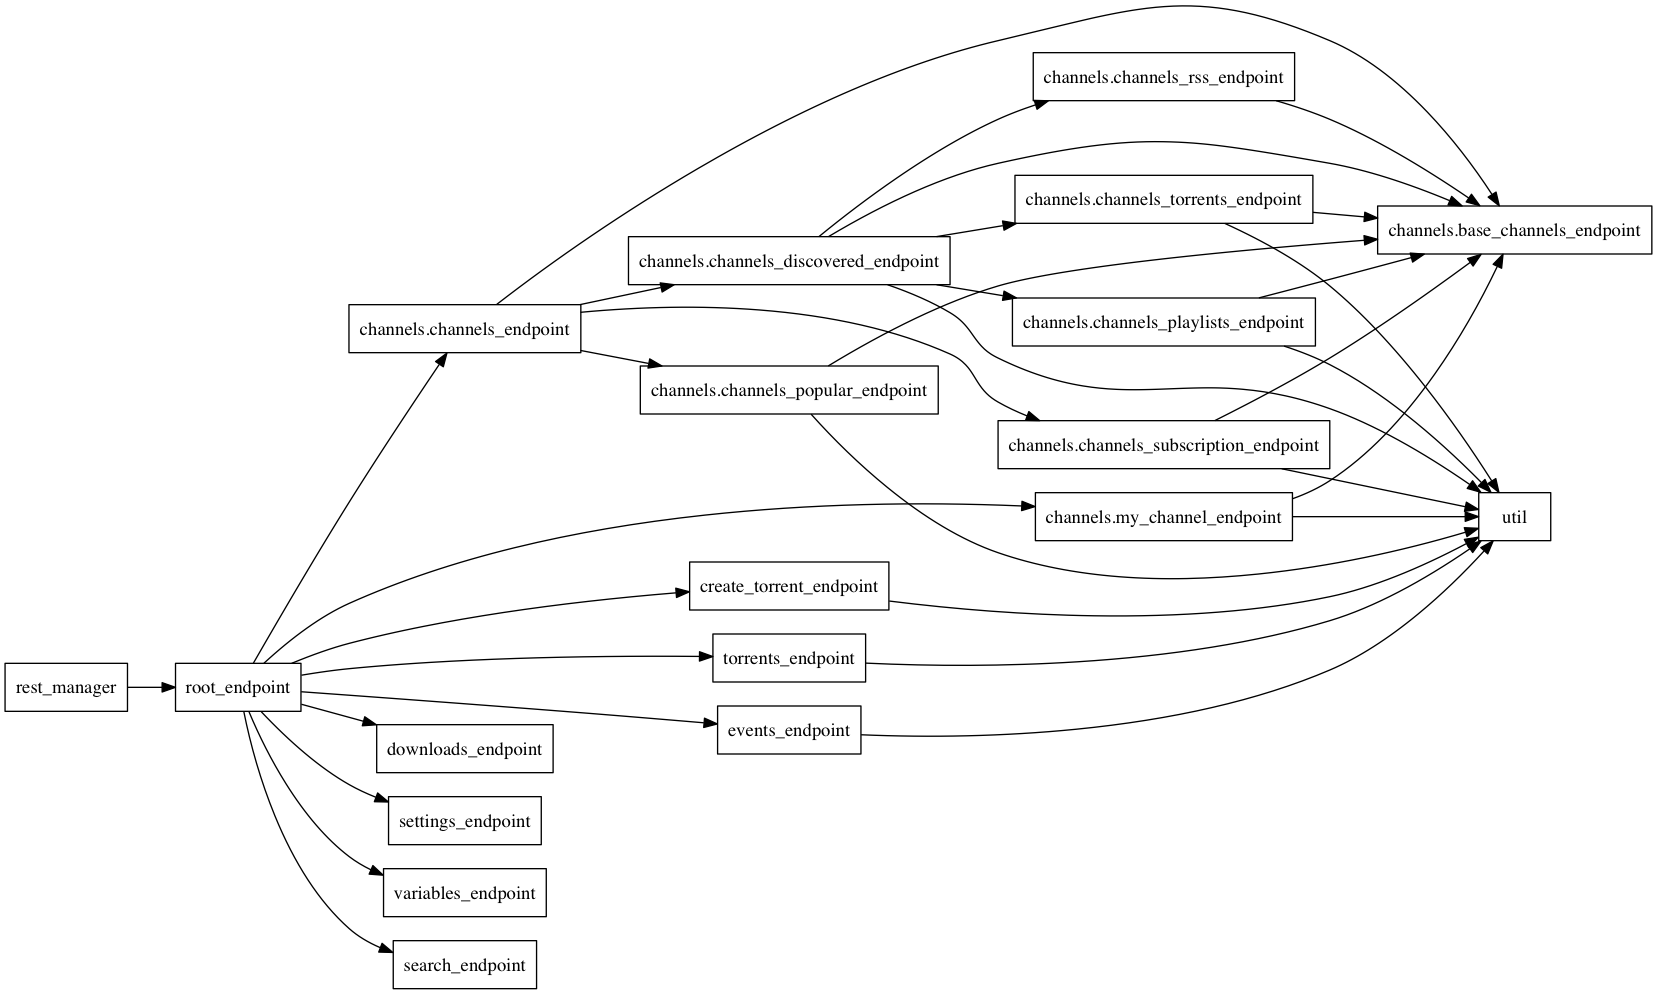
\includegraphics[width=1.0\columnwidth]{images/improving_qa/importgraph_api}
	\caption{The import graph of the REST API module.}
	\label{fig:importgraph-api}
\end{figure}

Except for some endpoints, all data returned by the API is structured in JSON format. The JSON format is well adopted in the field of web engineering and easy to parse. Most of the endpoints are straightforward implementations where the client performs a request and some data is returned. There are situations where the client does a request and a stream of data should be returned. For instance, this is the case when the user performs a search query. Sometimes, data should be returned to the client, even if the client did not ask for this data. When a crash in the Tribler core code occurred, the client should be notified of this crash and possibly warn the user that he or she should restart the application. For this purpose, an asynchronous events stream has been designed and created. Clients can open this event stream and interesting notifications are sent over this stream. All messages that are sent over the \emph{events} connection are shown in Table \ref{table:rest-api-events}.\\

\begin{table}
\begin{tabularx}{\textwidth}{|l|X|}
	\hline
	\textbf{Event name} & \textbf{Description} \\ \hline
	\emph{events\_start} & The events connection is opened and the server is ready to send events.  \\ \hline
	\emph{search\_result\_channel} & Tribler received a channel search result (either remote or locally). The event contains the channel result data. \\ \hline
	\emph{search\_result\_torrent} & Tribler received a torrent search result (either remote or locally). The event contains the torrent result data. \\ \hline
	\emph{upgrader\_started} & The Tribler upgrader started. \\ \hline
	\emph{upgrader\_tick} & The status of the Tribler upgrader changed. This event contains a human-readable string with the status update. \\ \hline
	\emph{upgrader\_finished} & The Tribler upgrader finished. \\ \hline
	\emph{watch\_folder\_corrupt\_torrent} & The watch folder module has encountered a corrupt .torrent file. The name of the file is part of this emitted event.\\ \hline
	\emph{new\_version\_available} & A new version of Tribler is available. The version number is contained in the event.\\ \hline
	\emph{tribler\_started} & Tribler has completed the startup procedure and is ready to serve HTTP requests on all endpoints.\\ \hline
	\emph{channel\_discovered} & A new channel has been discovered. The events contains the discovered channel data.\\ \hline
	\emph{torrent\_discovered} & A new torrent has been discovered. The events contains the discovered torrent data.\\ \hline
\end{tabularx}
\caption{An overview of all events that are passed over the asynchronous events connection, part of the REST API.}
\label{table:rest-api-events}
\end{table}

The API is started in two stages. Just before starting Tribler, the \emph{events} connection is activated. This connection is initialized earlier so we can send interesting updates of the upgrader to the client. When the upgrader is completed and Tribler has been started, the other endpoints are activated and the API is ready to be used.

\section{Graphical User Interface}
The amount of accumulated technical debt in the current graphical user interface of Tribler is devastating. After going through several development cycles where some impacting changes have been made, the code base of the user interface has reached the point where it is more beneficial to create a complete new user interface. This section will continue the discussion that has been initiated in Section \ref{chapter:problem-description}. First, the structure of the current user interface will be described. Next, the new interface, introduced in Chapter \ref{chapter:architecture} will be elaborated. Encountered design decisions and challenges are presented and discussed.

\subsection{The current user interface}
\todo{Better title} The current user interface is unintuitive and cluttered with widgets and many functionality that should be in the core module of Tribler, can be found at higher levels in the user interface code. There is actually no clear separation between the core and the user interface, making it hard for developers to develop and test new functionalities since they have to deal with a bigger code base. One of the goals of this thesis is to make this separation more explicit for developers so they do not have to touch interface-related code if they are not interested in that.\\\\
The code base of the user interface is full of code smells and undesired workarounds. There is no clear, documented structure. There are several reasons for that. One of the underlying reasons for this is the mindset of developers that the user interface code base is subordinate to the code related to the core functionalities of Tribler. While it is often true that minor defects in the user interface are less critical than errors in important core functionalities, developer should always strive to write maintainable code. The fact that the user interface has undergone dramatic changes throughout the 10 years of research is the second reason that led to the unstructured code base. Making short-term decisions were clearly favoured over decisions that benefit the longer-term development process.\\\\
If we take a closer look at the structure of the user interface code base, we see that there is no clear architecture or design. Several files with many class definitions can be found. In the \emph{widgets.py} file, we can identify 30 different widget definitions. The \emph{SearchGridManager} file acts like the glue between the Tribler core and the user interface. Most of the requests to the core are passing through method definitions inside this file.

\subsection{Building a new user interface}
Before starting to create a new user interface, we should first decide which graphical user interface library we would like to use. There are plenty of libraries that are suited for this job. Below, several of such libraries are summarized, together with a small description and some (dis)advantages.
\begin{itemize}
	\item \emph{wxPython}: this is the current user interface library we are using. \emph{wxPython} is built upon \emph{wxWidgets} and provides the Python bindings to this latter library. The library is cross-platform and we can continue to use \emph{wxPython}. We already have a large code base written in \emph{wxPython} so continued usage of this library could allow us to reuse several widgets. The main disadvantages of this library are the minor inconsistencies across different platforms and the lack of a visual designer, requiring us to specify the complete layout in Python code.
	\item \emph{Kivy}: the cross-platform library Kivy has been used by Tribler research, particularly in the past attempts to run Tribler on Android\cite{de2014android}\cite{sabee2014tribler}. The decision of using Kivy for the new user interface enables us to reuse the interface logic on Android. The layout of Kivy can either be created in \emph{.kv} files or specified in code which is based on the separation of concerns principle. While not as old as \emph{wxPython} or \emph{pyQt}, the library has gained significant attention and adoption in the Python community.
	\item \emph{TKinder}: the \emph{TKinder} library is a layer built upon the Tcl/Tk framework and is considered the de-facto graphical user interface library for Python. Like the other discussed frameworks, \emph{TKinder} does not provide a visual designer. The library is built-in in Python which means that no additional libraries have to be installed in order to start writing code. \emph{TKinder} however is considered more suitable for simple applications due to the simplistic nature of the library.
	\item \emph{PyQt}: \emph{PyQt} provides the Python bindings for the Qt framework and is widely used in open-source and commercial applications. With a first version released in 1995, the Qt framework has evolved into a mature state. The library is very well documentation and provides many different addons and plugins to support a wide range of applications. One of these plugins is a visual WYSIWYG designer where the layout of an interface can be specified in a drag-and-drop manner. This generates a \emph{xml} file which can be read and parsed by \emph{Qt}. Visual styles can be specified using the  \emph{Cascading Style Sheet} (CSS) language. The documentation of \emph{Qt} is very comprehensive, although the documentation regarding \emph{PyQt} is somewhat less maintained.
\end{itemize}
Since the graphical user interface will be an important aspect of Tribler, we wish to use a library that is future-proof, well-maintained and easy to use. We think that in the context of this thesis, choosing \emph{PyQt} is the best choice to build a new user interface. The fact that we can specify our layout using an editor is an enormous advantage since this will mean that we have less code to contribute. In addition, this allows other developers that are not familiar with the Tribler code base to contribute to the graphical user interface. The \emph{Qt} visual designer also offers tools for internationalization and translation of the interface in foreign languages. Tasks like these are perfect opportunities for contributions in an open source project and can potentially attract new developers. A screenshot of the used visualizer is visible in Figure x.\\\\
The result of the development of the new interface is displayed in Figure \ref{fig:new-gui-1}. The majority of the new user interface has been built using the visual designer. Some code has been written to handle requests to the Tribler core, display the right data in lists and to manage interface-related settings. Connections between widgets and Python code are made using the signal-slot mechanism in \emph{Qt}. This mechanism is used for communication between objects and is a central feature in the \emph{Qt} framework. Widgets in \emph{Qt} can have signals, events they want to possibly notify to other widgets. Some widgets have some built-in signals, i.e. a button emits a \emph{clicked} signal if the user clicks the button with the mouse. Other widgets or Python objects can subscribe to these signals. These signals and slots can either be specified using code or the visual designer, however, to keep the amount of Python code to be maintained to a minimum, we decided to specify our widgets connections in the visual designer as much as possible.\\

\begin{figure}[t]
	\centering
	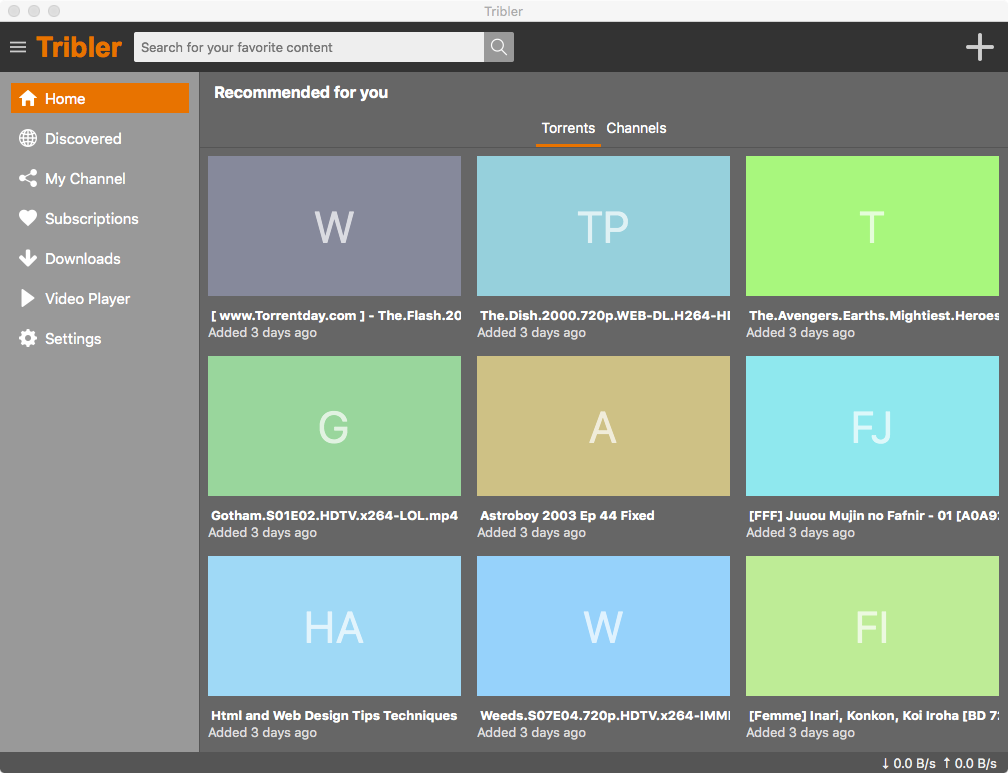
\includegraphics[width=0.8\columnwidth]{images/improving_qa/newgui1}
	\caption{The home page of the new user interface.}
	\label{fig:new-gui-1}
\end{figure}

During development of the user interface, some issues that required some careful analysis were encountered. The remained of the Section will describe these issues in more detail.

\begin{figure}[h!]
	\centering
	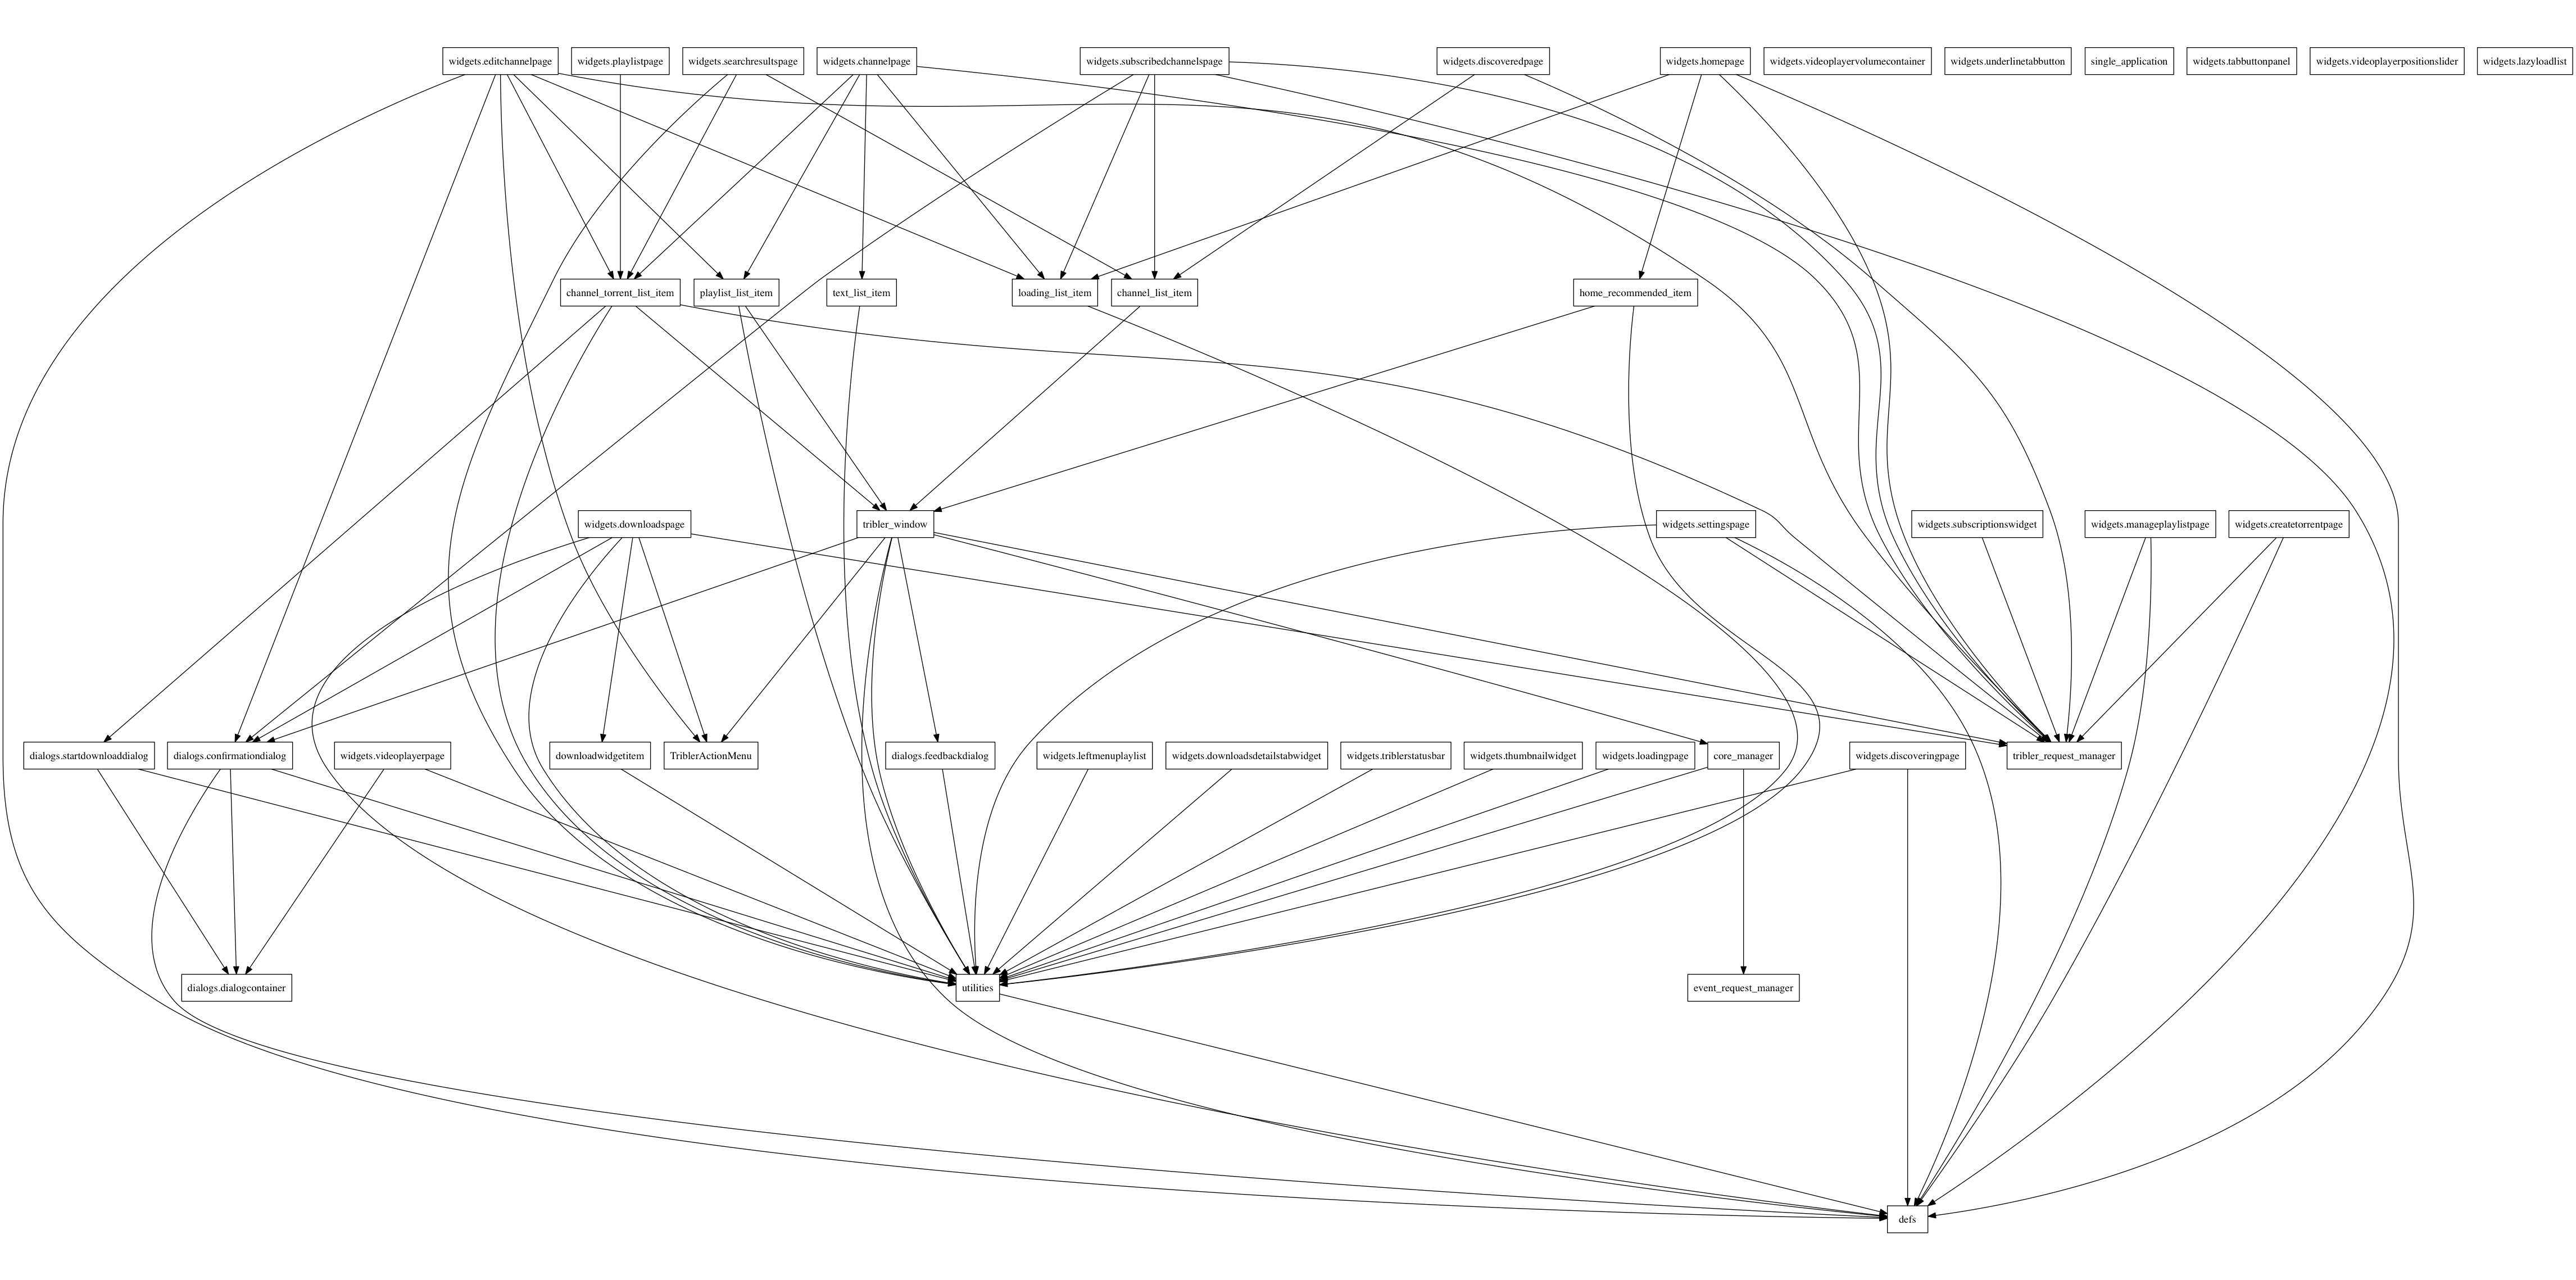
\includegraphics[width=1.0\columnwidth]{images/improving_qa/importgraph_new_gui}
	\caption{The generated import graph of the code base related to the new user interface.}
	\label{fig:importgraph-qt-gui}
\end{figure}

\subsubsection{\textbf{Displaying a huge amount of items}}
\emph{Qt} allows to display possibly many items in a simple list. The performance decreases dramatically if custom widgets are rendered in a list, like we are doing. Loading 1.000 of such list items takes several seconds\todo{verify this}. Channels hold potentially several thousand of torrents which should be displayed in the user interface. This problem can be solved by using lazy-loading techniques where more data is loaded when the user has scrolled through the end of the list. This solution has also been implemented in the interface written in \emph{wxPython}. By loading only a subset of the list rows, the user experience can be increased since users don't have to wait until the whole list of items is loaded. The implementation of this lazy-loading solution is reusable and can be found in the \emph{lazyloadlist.py} source file.

\section{Improving Sofware Artifacts}
